\documentclass[12pt,a4paper]{article}
\usepackage[left=2cm,right=2cm,top=2cm,bottom=2cm]{geometry}
\usepackage[utf8]{inputenc}
\usepackage[T2A]{fontenc}
\usepackage{amsmath}
\usepackage{amssymb}
\usepackage{graphicx}
\usepackage[russian]{babel}
\usepackage{indentfirst}
\usepackage{listings}
\usepackage{xcolor}
\usepackage{hyperref}

\hypersetup{
  colorlinks=true,
  urlcolor= blue,
  citecolor=blue,
  linkcolor= blue,
}

\title{Отчет по лабораторным работам №3-4 по дисциплине "Математическая статистика"}
\author{Скворцов Владимир Сергеевич (5030102/10201)}
\date{\today}

\begin{document}

	\begin{titlepage}

		\Large

		\begin{center}
			Санкт-Петербургский \\ Политехнический университет Петра Великого

			\vspace{10em}

			\textbf{Отчет по лабораторным работам №3-4} \\
			\textbf{по дисциплине}\\
			"\textbf{Математическая статистика}"

			\vspace{2em}

		\end{center}

		\vspace{6em}

		\newbox{\lbox}
		\savebox{\lbox}{\hbox{Скворцов Владимир Сергеевич}}
		\newlength{\maxl}
		\setlength{\maxl}{\wd\lbox}
		\hfill\parbox{12cm}{
			\hspace*{3cm}\hspace*{-5cm}Студент:\hfill\hbox to\maxl{Скворцов Владимир Сергеевич\hfill}\\
			\hspace*{3cm}\hspace*{-5cm}Преподаватель:\hfill\hbox to\maxl{Баженов Александр Николаевич}\\
			\\
			\hspace*{3cm}\hspace*{-5cm}Группа:\hfill\hbox to\maxl{5030102/10201}\\
		}

		\vspace{\fill}

		\begin{center}
			Санкт-Петербург \\ 2024
		\end{center}

	\end{titlepage}

	\tableofcontents\newpage

	\section{Постановка задачи}

	\subsection{Боксплот Тьюки}

	Сгенерировать выборки размером 20 и 100 элементов. Построить для них боксплот Тьюки.

	\subsection{Доверительные интервалы для параметров нормального распределения}

	Сгенерировать выборки размером 20 и 100 элементов. Вычислить параметры положения и рассеяния:

	\begin{itemize}
		\item для нормального распределения,
		\item для произвольного распределения.
	\end{itemize}

	\section{Теоретическое обоснование}

	\subsection{Функции распределения}

	\begin{itemize}
		\item Нормальное распределение

		\begin{equation} \label{eq:normal}
			N(x, 0, 1) = \frac{1}{\sqrt{2\pi}}e^\frac{-x^2}{2}
		\end{equation}

		\item Распределение Коши

		\begin{equation} \label{eq:cauchy}
			C(x, 0, 1) = \frac{1}{\pi}\frac{1}{x^2+1}
		\end{equation}

		\item Распределение Стьюдента $t(x, 0, 3)$ с тремя степенями свободы

		\begin{equation} \label{eq:student}
			t(x, 0, 3) = \frac{6\sqrt3}{\pi(3 + t^2)^2}
		\end{equation}

		\item Распределение Пуассона

		\begin{equation} \label{eq:poisson}
			P(k, 10) = \frac{10^k}{k!}e^{-10}
		\end{equation}

		\item Равномерное распределение

		\begin{equation} \label{eq:uniform}
			U(x, -\sqrt3, \sqrt3) = \begin{cases}
				\frac{1}{2\sqrt3}, & \; |x| \leq \sqrt3\\
				0, & \; |x| > \sqrt3
			\end{cases}
		\end{equation}
	\end{itemize}

	\subsection{Боксплот Тьюки}

	Боксплот (англ. box plot) — график, использующихся в описательной статистике, компактно изобрадающий одномерное распределение вероятностей. Такой вид диаграммы в удобной форме показывает медиану, нижний и верхний квартили и выбросы. Границами ящика служат первый и третий квартили, линия в середине ящика — медиана. Концы усов — края статистически значимой выборки (без выброса). Длину <<усов>> определяют разность первого квартиля и полутора межквартальных расстояний и сумма третьего квартиля и полутора межквартальных расстояний. Формула имеет вид

	\begin{equation} \label{eq:box_plot}
		X_1 = Q_1 - \frac{3}{2}(Q_3 - Q_1), \ X_2 = Q_3 + \frac{3}{2}(Q_3 - Q_1),
	\end{equation}

	где $X_1$ — нижняя граница уса, $X_2$ — верхняя граница уса, $Q_1$ — первый квартиль, $Q_3$ - третий квартиль.
	Данные, выходящие за границы усов (выбросы), отображаются на графике в виде маленьких кружков.
	Выбросами считаются величины $х$, такие что:

	\begin{equation} \label{eq:outlier}
		\left[
			\begin{array}{ll}
					x < X_1^T \\
					x > X_2^T
			\end{array}
		\right .
	\end{equation}

	\subsection{Доверительные интервалы для параметров нормального распределения}

	Пусть $F_T(x)$ — функция распределения Стьюдента с $n - 1$ степенями свободы. Полагаем, что $2F_T(x) - 1 = 1 - \alpha$, где $\alpha$ — выбранный уровень значимости. Тогда $F_T(x) = 1 - \alpha / 2$. Пусть $st_{1 - \alpha / 2}(n - 1)$ — квантиль распределения Стьюдента с $n - 1$ степенями свободы и порядка $1 - \alpha / 2$. Тогда получаем

	\begin{equation} \label{eq:normal_mean_boundaries}
		P \left ( \overline x - \frac{st_{1 - \alpha / 2}(n - 1)}{\sqrt{n - 1}} < m < \overline x + \frac{st_{1 - \alpha / 2}(n - 1)}{\sqrt{n - 1}} \right ) = 1 - \alpha,
	\end{equation}

	что и даст доверительный интервал для m с доверительной вероятностью $\gamma = 1 \alpha$ для нормального распределения.

	Случайная величина $n \frac{s^2}{\sigma^2}$ распределена по закону $\chi^2$ с $n - 1$ степенями свободы. Тогда

	\begin{equation} \label{eq:mean_boundaries}
		P \left ( \overline x - \frac{st_{1 - \alpha / 2}(n - 1)}{\sqrt{n - 1}} < m < \overline x + \frac{st_{1 - \alpha / 2}(n - 1)}{\sqrt{n - 1}} \right ) = 1 - \alpha,
	\end{equation}

	\section{Описание работы}

	Лабораторные работы выполнены с использованием Python и его сторонних библиотек: \verb!numpy!, \verb!pandas!, \verb!matplotlib!, \verb!seaborn!.

	Ссылка на GitHub репозиторий: \href{https://github.com/vladimir-skvortsov/spbstu-mathematical-statistics}{https://github.com/vladimir-skvortsov/spbstu-mathematical-statistics}

	\newpage

	\section{Результаты}

	\subsection{Гистограммы и графики плотности распределения}

	\begin{figure}[htbp!]
		\begin{center}
			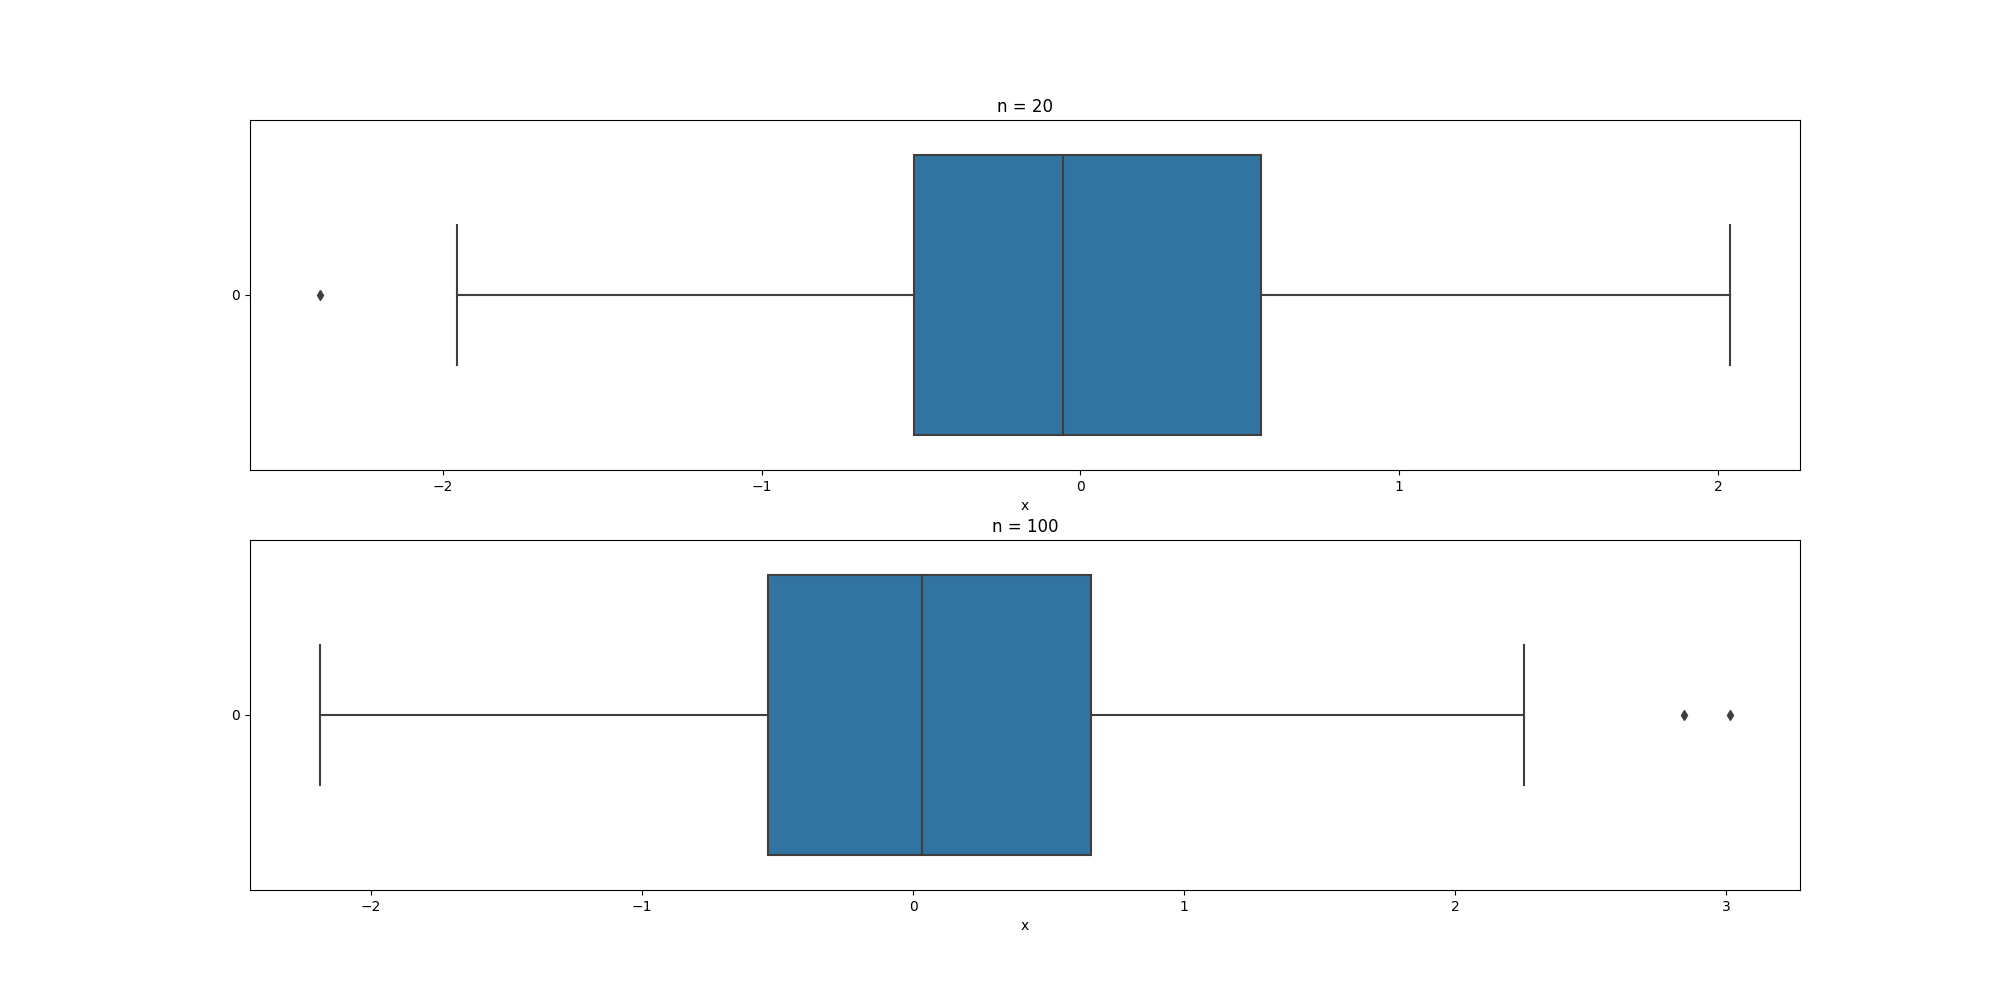
\includegraphics[width = 1.12\linewidth]{graphics/normal.png}
			\caption{Нормальное распределение \ \eqref{eq:normal}}
		\end{center}
	\end{figure}

	\begin{figure}[htbp!]
		\begin{center}
			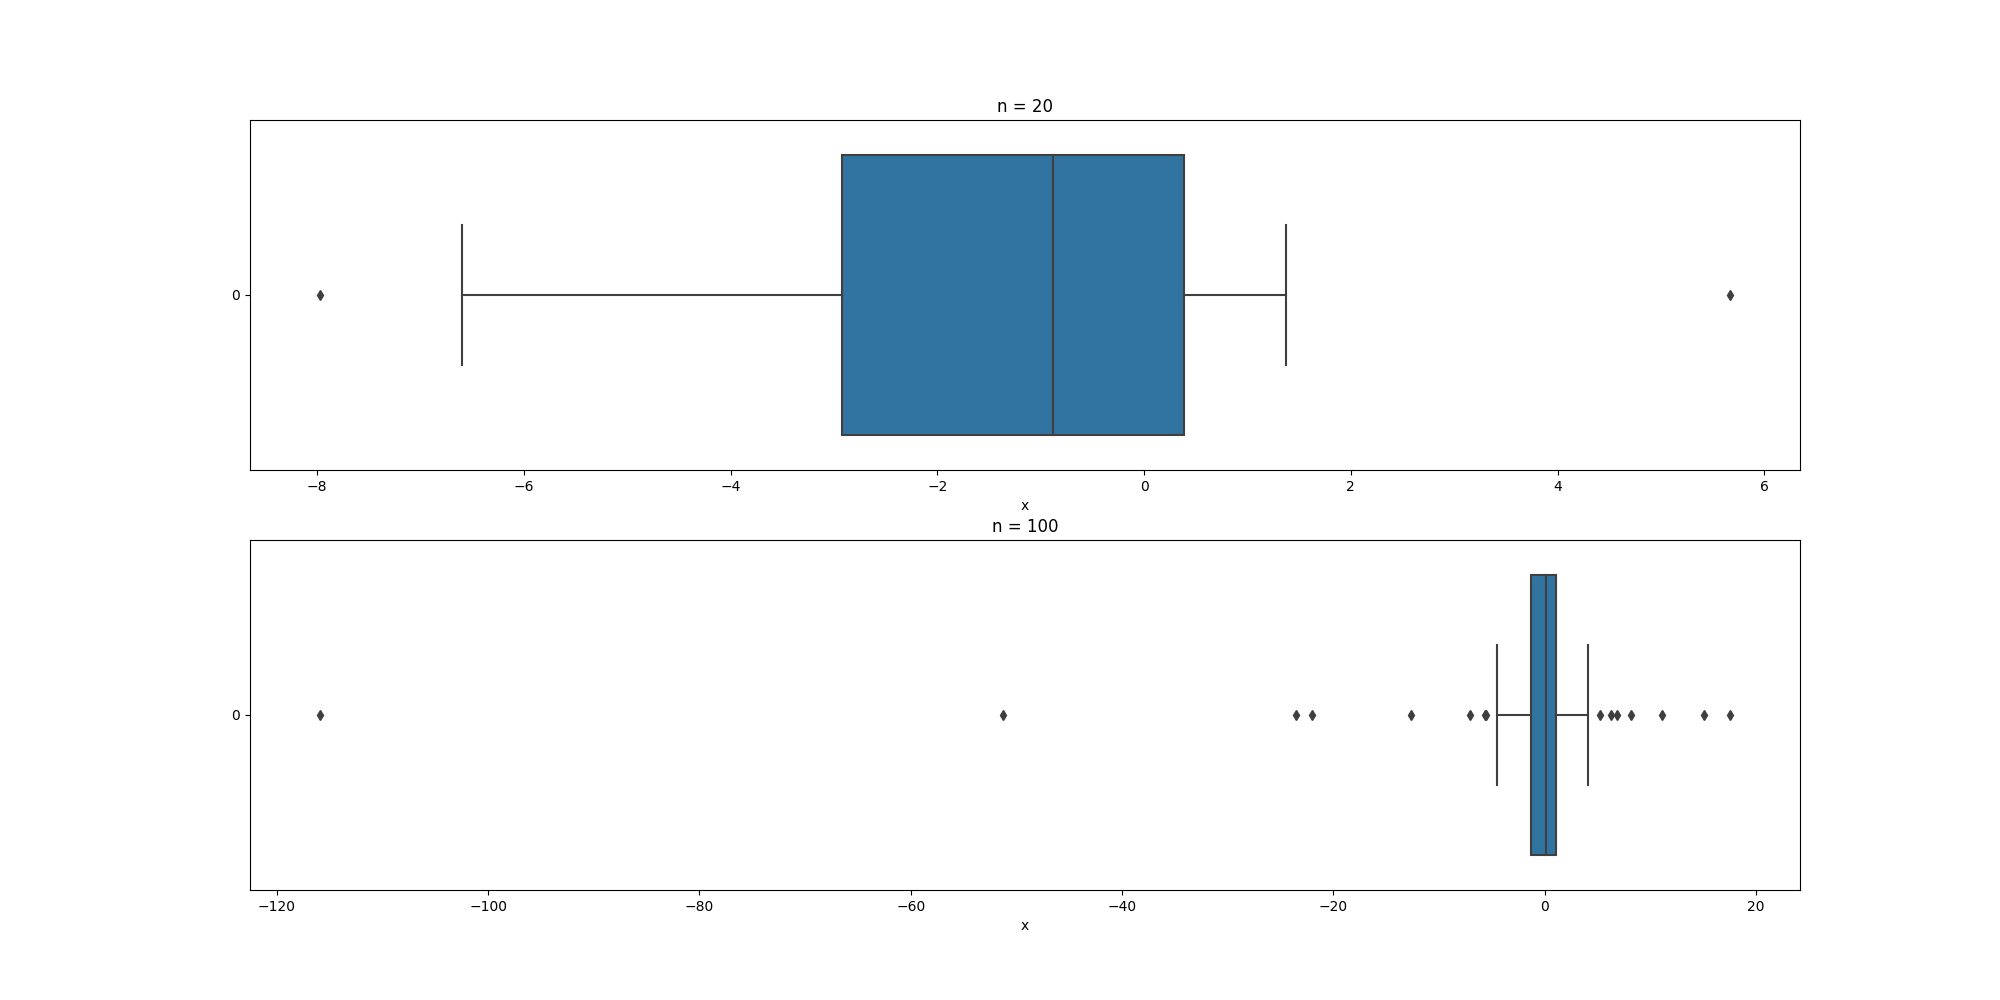
\includegraphics[width = 1.12\linewidth]{graphics/cauchy.png}
			\caption{Распределение Коши \ \eqref{eq:cauchy}}
		\end{center}
	\end{figure}

	\newpage

	\begin{figure}[htbp!]
		\begin{center}
			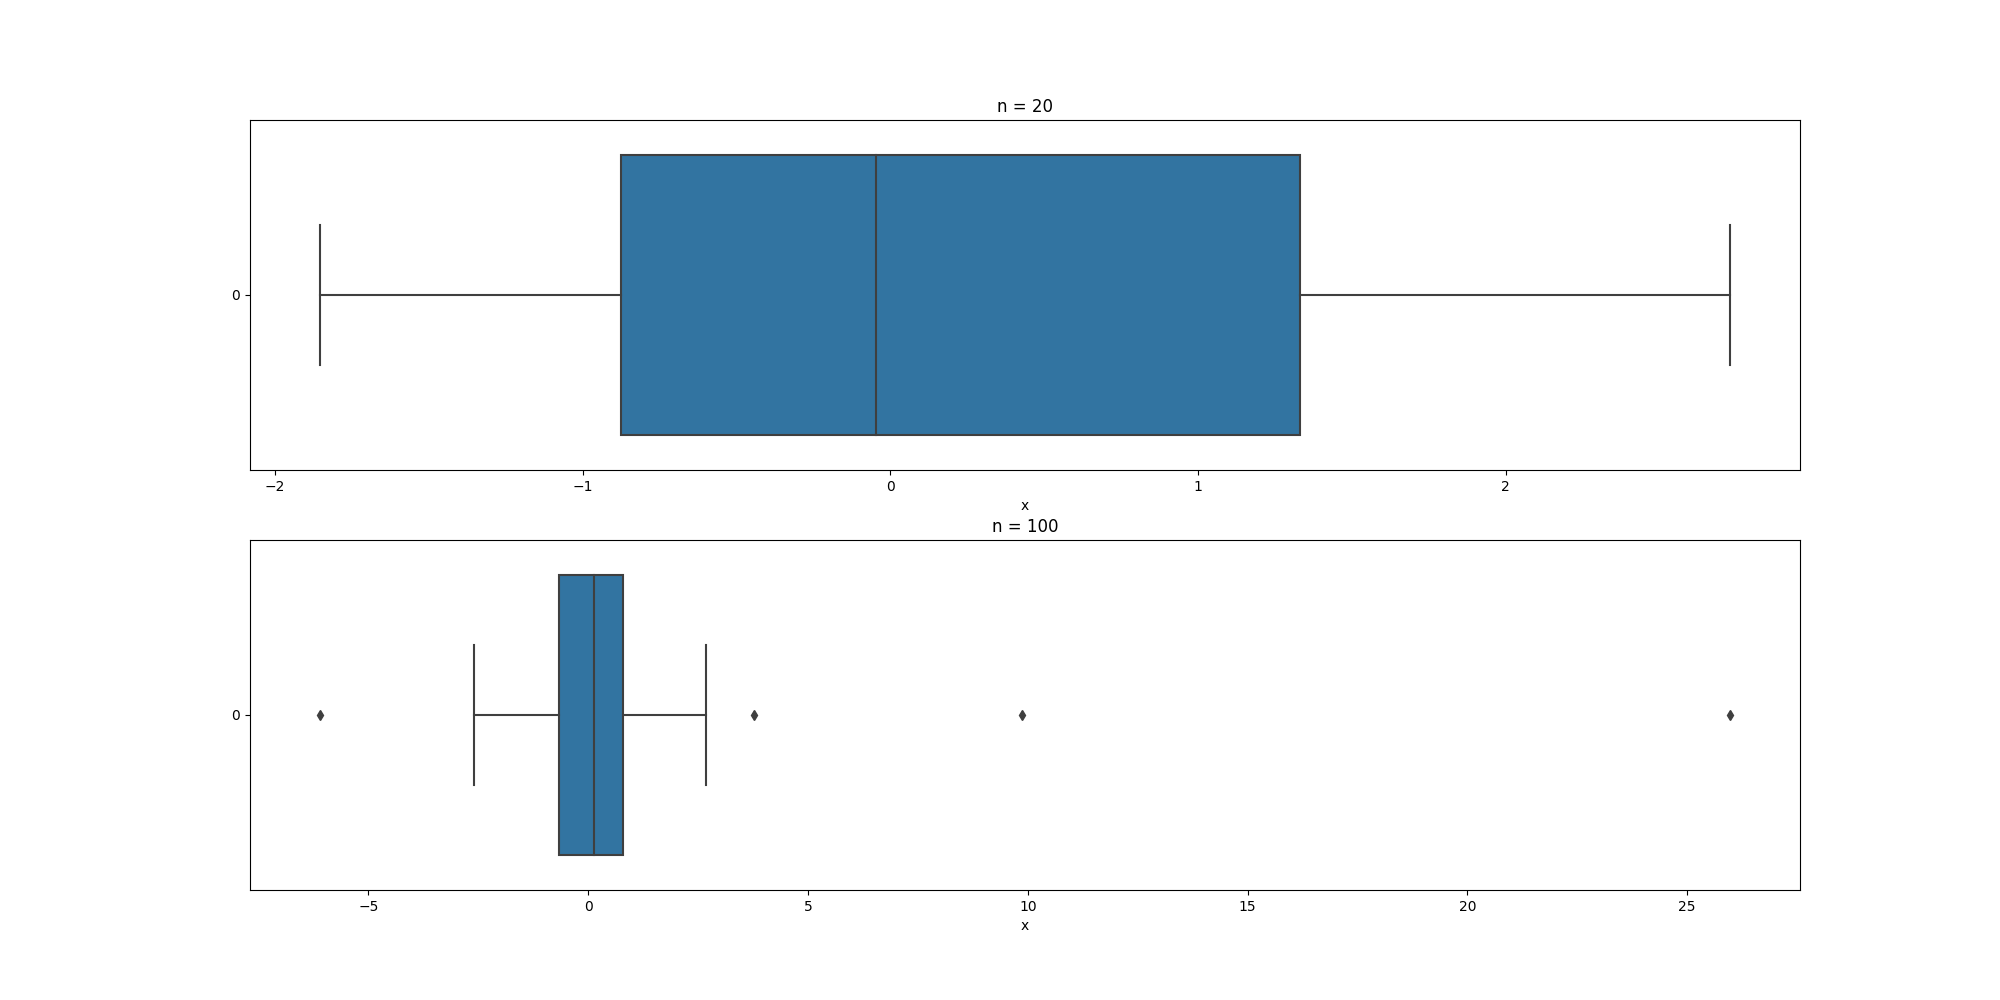
\includegraphics[width = 1.12\linewidth]{graphics/student.png}
			\caption{Распределение Стьюдента \ \eqref{eq:student}}
		\end{center}
	\end{figure}

	\begin{figure}[htbp!]
		\begin{center}
			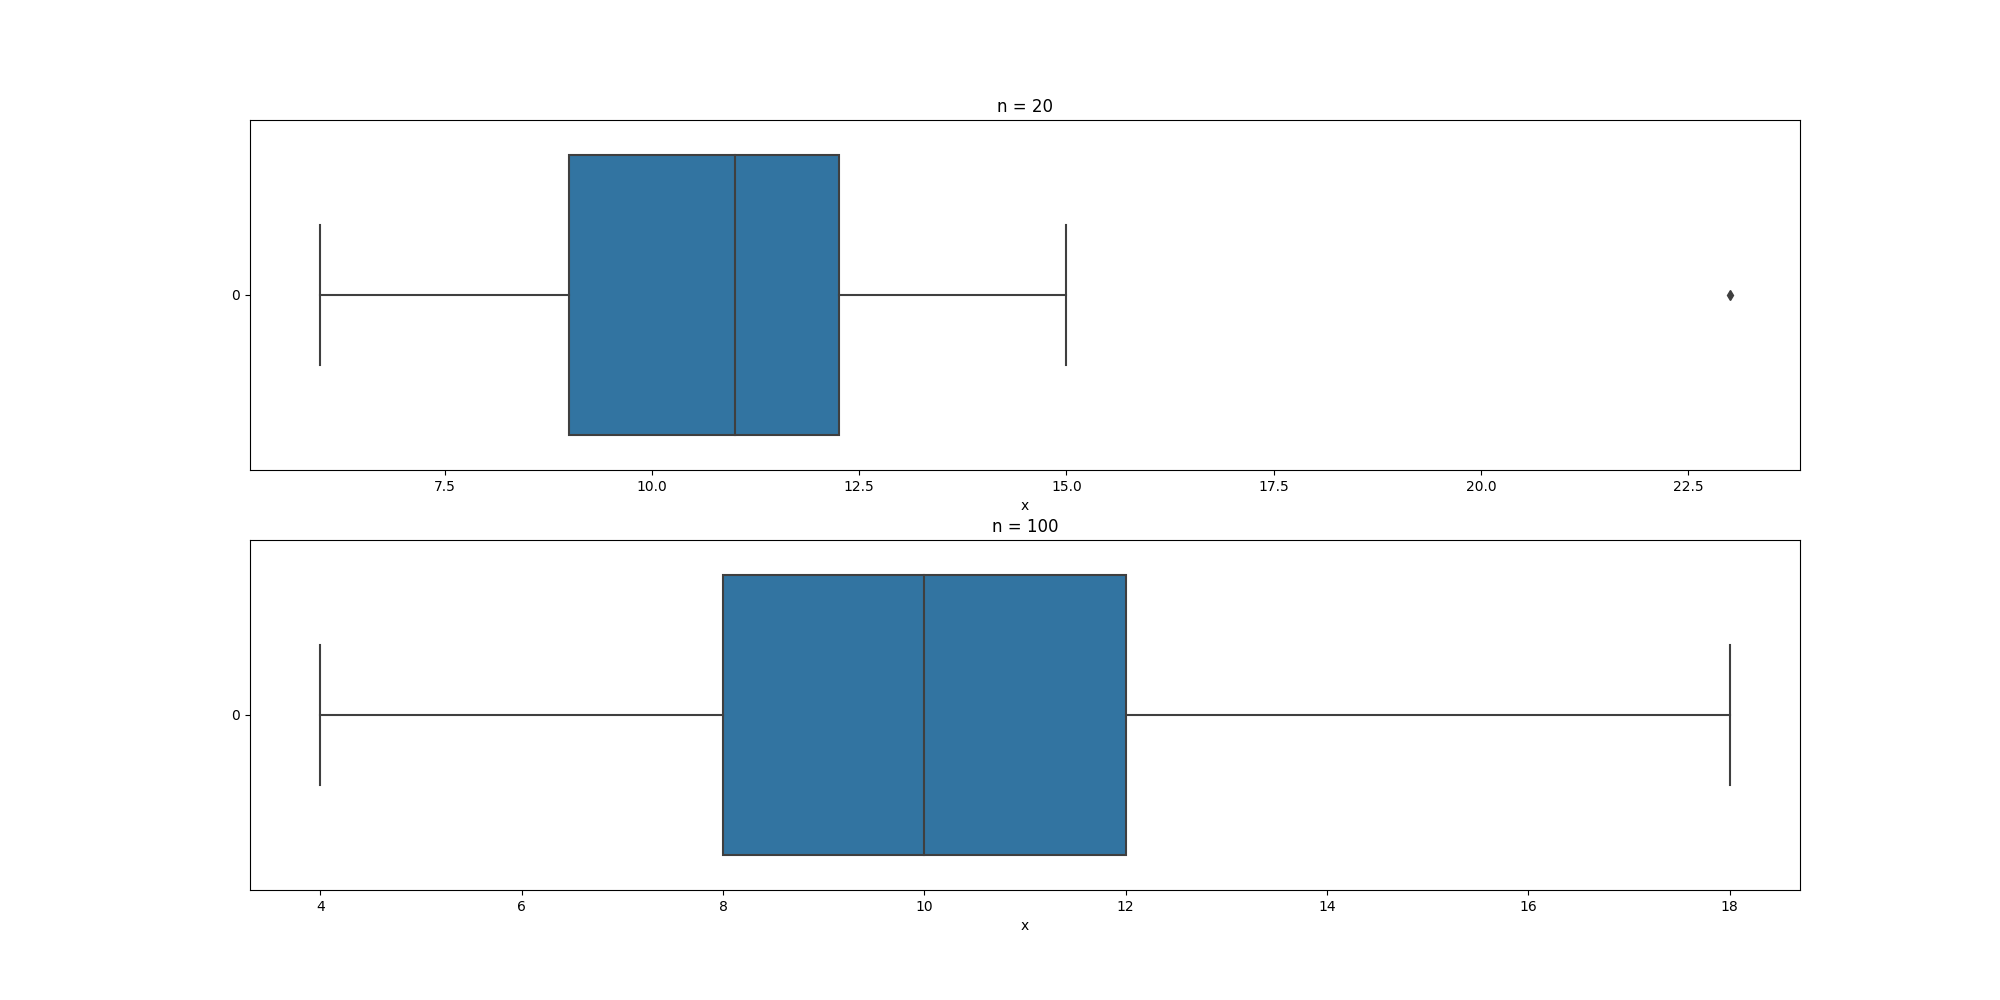
\includegraphics[width = 1.12\linewidth]{graphics/poisson.png}
			\caption{Распределение Пуассона \ \eqref{eq:poisson}}
		\end{center}
	\end{figure}

	\begin{figure}[htbp!]
		\begin{center}
			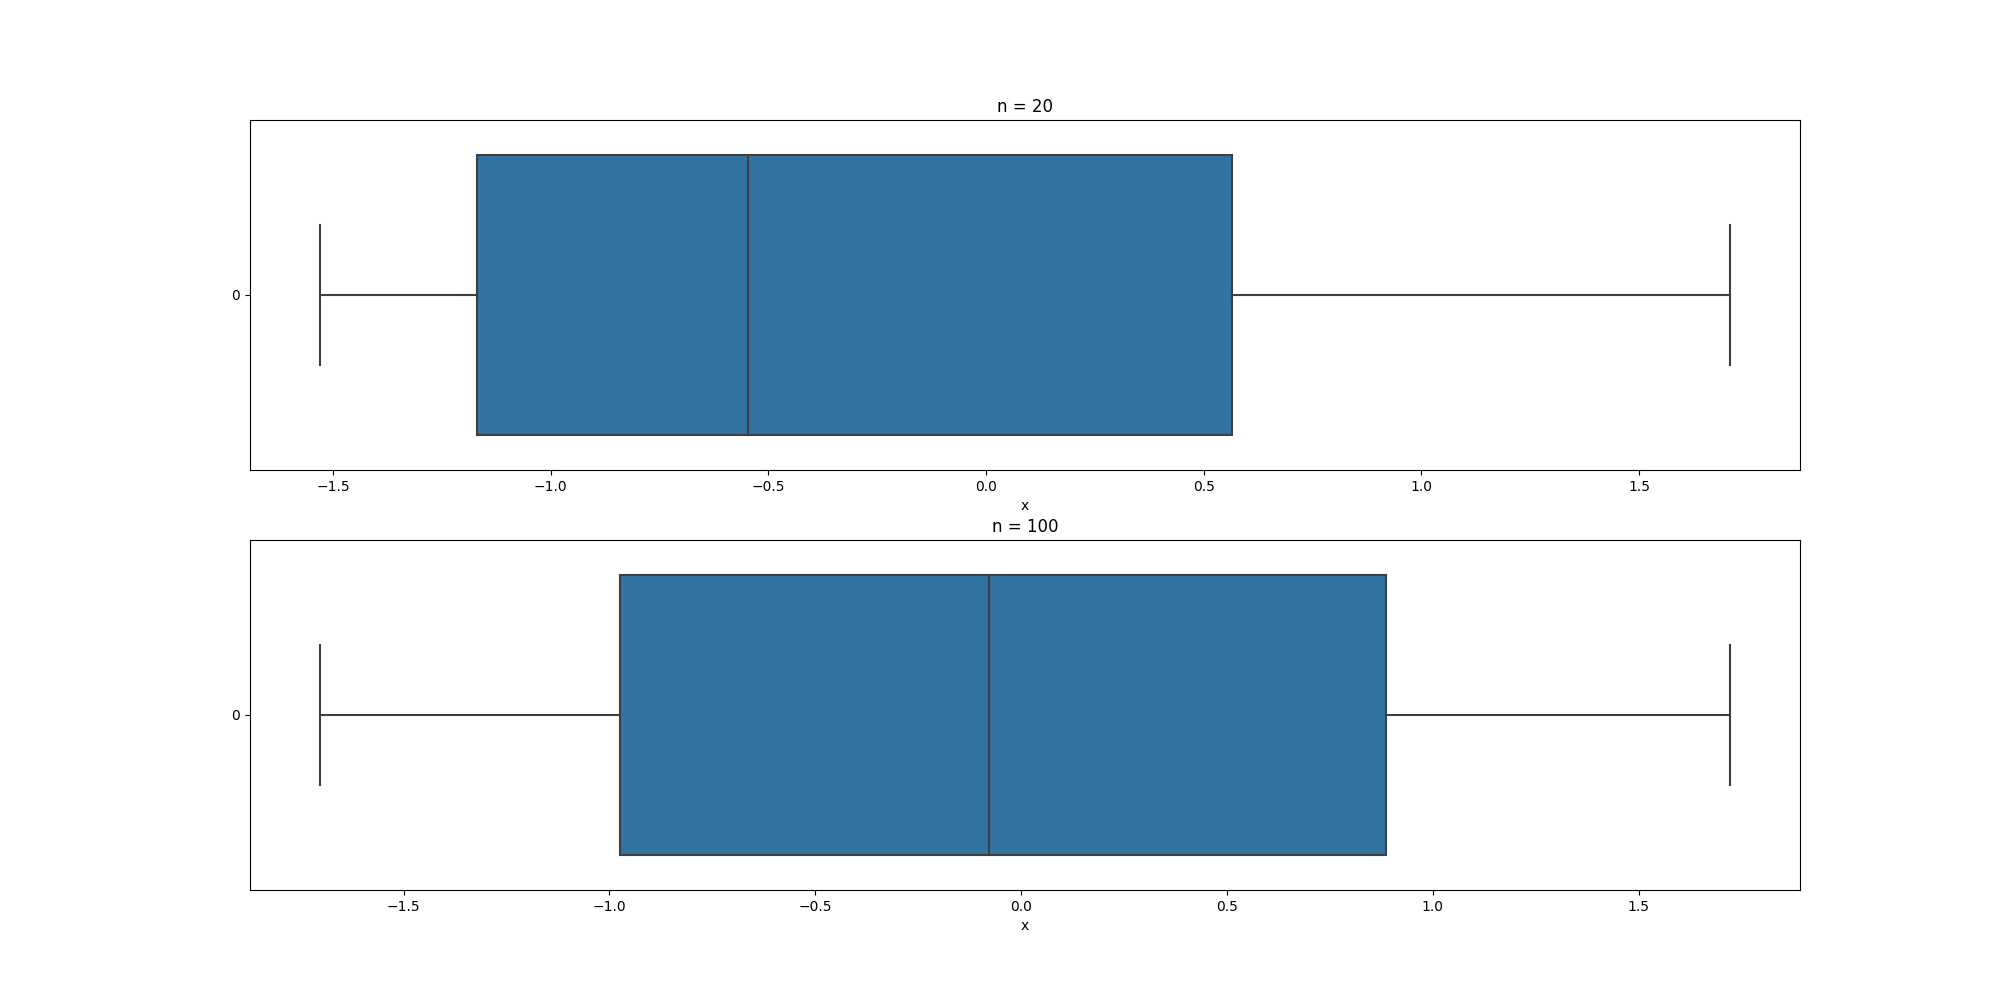
\includegraphics[width = 1.12\linewidth]{graphics/uniform.png}
			\caption{Равномерное распределение \ \eqref{eq:uniform}}
		\end{center}
	\end{figure}

	\newpage

	\subsection{Доверительные интервалы для параметров распределений}

	\begin{table}[htbp!]
		\centering
		\begin{tabular}{ |c|c|c| }
			\hline
			n = 20 & m & $\sigma$ \\
			\hline
			& -0.43 < m < 0.37 & 0.66 < $\sigma$ < 1.25 \\
			\hline
			n = 100 & m & $\sigma$ \\
			\hline
			& -0.12 < m < 0.24 & 0.81 < $\sigma$ < 1.07 \\
			\hline
		\end{tabular}
		\caption{Доверительные интервалы для параметров нормального распределения \eqref{eq:normal}}
		\label{table:1}
	\end{table}

	\begin{table}[htbp!]
		\centering
		\begin{tabular}{ |c|c|c| }
			\hline
			n = 20 & $m$ & $\sigma$ \\
			\hline
			& 0.11 < $m$ < 0.97 & 0.29 < $\sigma$ < 0.33 \\
			\hline
			n = 100 & $m$ & $\sigma$ \\
			\hline
			& 0.30 < $m$ < 0.67 & 0.28 < $\sigma$ < 0.33 \\
			\hline
		\end{tabular}
		\caption{Доверительные интервалы для параметров произвольного распределения. Асимптотический подход}
		\label{table:2}
	\end{table}

	\begin{figure}[htbp!]
		\begin{center}
			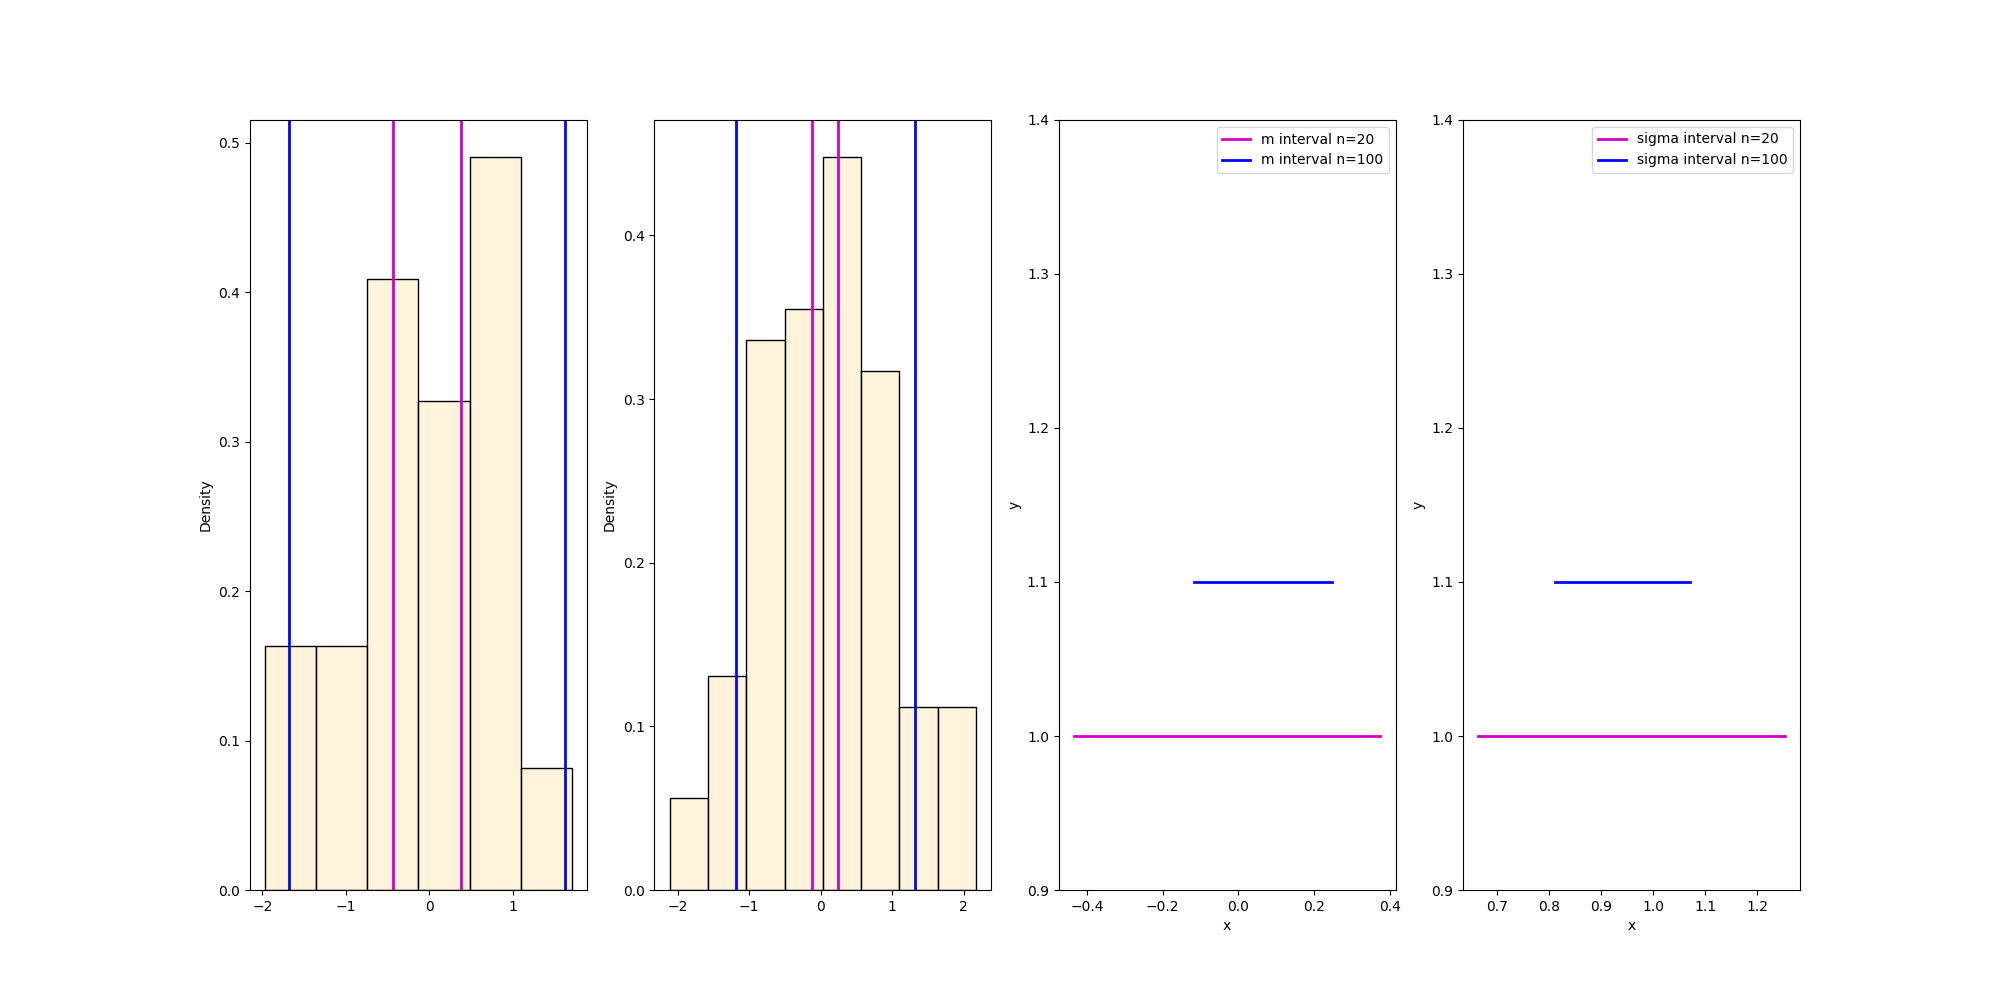
\includegraphics[width = 1.12\linewidth]{graphics/hists.png}
			\caption{Гистограммы и оценки для параметров нормального распределения}
		\end{center}
	\end{figure}

	\vspace{10em}

	\section{Выводы}

	По результатам выполнения лабораторной работы были сгенерированы выборки размером 20 и 100 элементов и построены для них боксплоты Тьюки.

	Боксплот позволяет наглядно представить основные характеристики выборки - медиану, квартили, межквартальный размах и выбросы. На основе построенных графиков можно увидеть разницу в распределении данных для двух выборок. Для выборки размером в 100 элементов представленные метрики имеют более проработанный вид, ведь с увеличением размера выборки улучшается точность оценок параметров распределения.

	Также в ходе выполнения лабораторной работы были сгенерированы две выборки размерами 20 и 100 элементов для нормального и произвольного распределения. Затем для каждой из них были вычислены параметры распределения: среднее значение и дисперсия.

	Результаты, представленные графически, демонстрируют, что количество элементов в выборке влияет на точность оценок параметров. Более большое количество наблюдений (т.е. 100 элементов) приводит к более точным и стабильным оценкам среднего и дисперсии, как для нормального, так и для произвольного распределения. Для выборки с меньшим количеством элементов (20 элементов) оценки могут сильно варьироваться в зависимости от конкретной выборки, что также наглядно отображено на графиках.

	Лабораторная работа иллюстрирует важнейший статистический принцип: точность статистической оценки увеличивается с ростом объема выборки. Результаты этого исследования подчеркивают значимость использования достаточно больших выборок для надежного анализа данных.
\end{document}
